\section{Parabolic induction and Hilbert modules}

Here is a question formulated by Pierre Julg. \\

Let $G$ be a real reductive group. For all parabolic subgroup $P$, there is only one nilpotent normal subgroup $N$, and the Levi is defined as $P=LN$. The idea of Pierre Julg is to fix first a Levi susgroup $L$ of $G$. Now there is only a finite numbers of choices for $N$, so that
\[P(L)=\left\{N : P=LN \text{ is parabolic}\right\}\]
is a finite set. The Weyl group $W_L = N_G(L)/L$ acts on it by $w.N = wNw^{-1}$.\\
Pierre Clare defined a $C^*_r L$-module $C^*_r(G/N)$, equipped with and action of $C^*_r G$ by compacts operators. He was able to give a nice interpretation of parabolic induction in terms of functors on these modules. Let $(\sigma,\tau)\in \hat{M_d}\times \hat A$, where $L=MA$, $\hat{M_d}$ is the discrete dual of $M$, and $\hat A = \mathfrak a^*$. Then $\sigma\otimes \tau$ is a représentation of $MA=L$, which we can trivially extend to $N$ to induce it on $G$. Pierre Clare showed the following fact :

\[Ind_P^G \ H_{\sigma\otimes\tau\otimes 1_N} = C^*(G/N)\otimes_{C^*_rL} H_{\sigma\otimes\tau}.\] 

For every $\tilde w\in N_G(L)$, the operator $\rho(\tilde w) : C_r^*(G/N)\rightarrow C_r^*(G/w.N)$ is well defined and gives a morphism
\[Ad \ \rho(\tilde w) : \mathfrak K_{C_r^*L}(C_r^*(G/N)\rightarrow \mathfrak K_{C_r^*L}(C_r^*(G/w.N))\] 
because $C_r^*G$ is acting on $C^*(G/N)$ by compact operators. This gives a morphism
\[C^*_r G \rightarrow \bigoplus_{[L]} \left(\bigoplus_{N\in P(L)} \mathfrak K(C^*_r(G/N))\right)^{W_L}\] 
which Pierre Julg conjectures to be an isomorphism. (This is true but due to very hard work in Harish-Chandra's theory, the aim is to find a relatively easy proof using standard $C^*$-algebraic tools).\\

The first step would be to prove that 
\[\begin{array}{rcl}C^*_r G & \rightarrow & \left(\bigoplus_{N\in P(L)} \mathfrak K(C^*_r(G/N))\right)^{W_L}\\
f &\mapsto & (\pi_N(f))\end{array}\] 
is surjective, using Fourier transform and a conjectural formula, 
\[\pi_N(F^{-1}_N(T))=\frac{1}{\# W_L}\sum w.T,\]
 for $F^{-1}_N(g)=\text{Tr}_{C_d^*L}\ (T\pi_N(g^{-1}))$.

\subsection{In $SL(2,\R)$}

In this case, $G$ acts on the Poincaré disc by homographies, and $P$ can be taken as the stabilizer of a point at infinity, and $L$ stabilizes a geodesic, that is to say two points at infinity, so that
\[P_{1,1}\simeq\{\begin{pmatrix}a & * \\ 0 & a^{-1}\end{pmatrix}\},\quad
L\simeq\{\begin{pmatrix}a & 0\\ 0 & a^{-1}\end{pmatrix}\},\quad
N\simeq\{\begin{pmatrix}1 & * \\ 0 & 1\end{pmatrix}\},\quad
W_L\simeq \Z_2.
\]

Here Julg's point of view applies directly : fixing $P$ amounts to fix a point at infinity, which gives infinite choices for the second point giving the geodesic and $L$. Now fix two points at infinity, which gives you $L$. You now only have two choices for $P$, and the two are exchanges under the action of $W_L$ on the nilpotent groups.\\

\begin{figure}[h]\centering
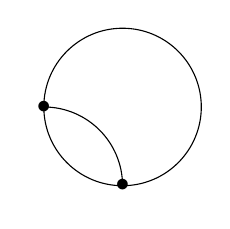
\begin{tikzpicture}
\draw (0,0) circle (1) ;
\draw (0,-1) arc (0:90:1);
\draw (0,-1) node {$\bullet$};
\draw (-1,0) node {$\bullet$};
\end{tikzpicture}
\caption{Choices for the Levi subgroup}
\label{fig:Levi}
\end{figure}






















